% Chapter 2

\chapter{Adiabatic quantum computing} % Main chapter title

\label{Chapter2} % For referencing the chapter elsewhere, use \ref{Chapter1} 
In the present chapter we show a paradigm of quantum computation known as \textit{adiabatic quantum computing} (AQC), see Ref. \cite{Farhi2000QuantumEvolution}. We start by sketching the rough idea of the adiabatic theorem to finally derive a formal proof of it. We also expose one application of AQC to solve \textit{quadratic unconstrained binary optimization} (QUBO) problems, known as \textit{quantum annealing} (QA), see Ref. \cite{Kadowaki1998QuantumModel}.

%%%%%%%%%%%%%%%%%%%%%%%%%%%%%%%%%%%%%%%%%%%%%%%%%%%%%%%%%%%%%%%%%%%%%%%%%%%%%%%%%%%%%%%%%%%%%%%%%%%%%%%%%%
%     1.1 ADIABATIC APPROXIMATION
%%%%%%%%%%%%%%%%%%%%%%%%%%%%%%%%%%%%%%%%%%%%%%%%%%%%%%%%%%%%%%%%%%%%%%%%%%%%%%%%%%%%%%%%%%%%%%%%%%%%%%%%%%
\section{The Adiabatic Theorem}
Quoting Sarandy and Lidar\,\cite{Sarandy2005AdiabaticSystems},
\begin{displayquote}
\textit{The theorem posits, roughly, that if a state is an instantaneous eigenstate of a sufficiently slowly varying Hamiltonian at one time, then it will remain an eigenstate at later times, while its eigenenergy evolves continuously.}
\end{displayquote}
\subsection{The adiabatic protocol}
We need to construct an initial Hamiltonian $\mathcal{H}(t=0) = \mathcal{H}_{i}$ whose ground state is known and whose time evolution, $t \in \left[0,T\right]$ -- where $T$ is the total evolution time -- leads to a Hamiltonian $\mathcal{H}(t=T) = \mathcal{H}_{f}$ that encodes the solution to our problem. Mathematically we can write a linear schedule between the initial and target Hamiltonian,
\begin{equation}
\label{eq:Htime}
    \mathcal{H}(t) = \left(1-\frac{t}{T}\right)\mathcal{H}_{i} + \left(\frac{t}{T} \right)\mathcal{H}_{f}
\end{equation}
The adiabatic theorem guarantees that if we start with an initial Hamiltonian $\mathcal{H}_{i}$ in a given eigenspace and the evolution is carried out sufficiently slowly -- in further sections we demonstrate what slowly means in detail -- then we end up in the equivalent eigenspace of the final Hamiltonian $\mathcal{H}_{f}$. \\\\
To summarise:
\begin{itemize}
    \item \textbf{Step 1 (Mapping):} Map the problem into a Hamiltonian $\mathcal{H}_{f}$. Typically, the problem is encoded in the ground state so do we.
    \item \textbf{Step 2 (Initialise $\mathcal{H}_{i}$):} Initialise the system in the ground state of a Hamiltonian $\mathcal{H}_{i}$, easy to compute and to experimentally prepare. For instance, the ground state of $\mathcal{H} = - \sum_{i}^{n}\hat{\sigma}_{i}^{x}$ is the eigenvector $\ket{+}^{\otimes n}$.
    \item \textbf{Step 3 (Adiabatic Theorem):} Slowly evolve the system from $H_{i}$ to $H_{f}$. The adiabatic theorem guarantees that, under certain conditions that will be explained later, the system will end up in the ground state of $H_{f}$.
    \item \textbf{Step 4 (Measure):} Measure the eigenstate of $H_{f}$. The result encodes a solution to our problem.
\end{itemize}
Notice that we wrote in the last step that the result of the measurement provides "a solution" not "the solution". This is because there are two possibilities for a finite-dimensional Hamiltonian:
\begin{itemize}
    \item \textbf{Non-degenerate Hamiltonian:} We start with an initial Hamiltonian $\mathcal{H}_{i}$ in its ground eigenstate $\ket{g(t=0)}$ and end up in the equivalent eigenstate -- ground state -- of the final Hamiltonian $\mathcal{H}_{f}$ where the eigenvalue is $E_{g}(t=T)$ and the eigenvector is\\
    $\ket{g(t=T)}$.
    \item \textbf{Degenerate Hamiltonian:} We start with an initial Hamiltonian $\mathcal{H}_{i}$ in its ground eigen-\\
    space spanned by $\{\ket{g^{i}(t=0)}\}_{i \in \left[1,d\right]}$, where $d$ is the degeneracy of the ground state, and end up in the equivalent eigenspace of the final Hamiltonian $\mathcal{H}_{f}$ with eigenvalue $E_{g}(t=T)$.
\end{itemize}
Intuitively, one can think that a problem can have multiple configurations that lead to the same minimum eigenvalue.
%%%%%%%%%%%%%%%%%%%%%%%%%%%%%%%%%%%%%%%%%%%%%%%%%%%%%%%%%%%%%%
\subsection{The Adiabatic Theorem: A First Approach}
We now provide a simple argument to build intuition into the adiabatic theorem. The next section will be devoted to a formal proof. In order to continue, let us define the following dimensionless variable
\begin{equation}
    s \equiv \frac{t}{T}\, , \quad s \in [0,1]
\end{equation}
For instance, consider a discrete and non-degenerate $n$-qubit system. A state of that system can be written as a linear combination of the instantaneous eigenstates of the Hamiltonian $\ket{\psi(s)} = \sum_{i}c_{i}(s)\ket{i(s)}$ as function of $s$. Its evolution is given by the time-dependent Schrödinger equation, see Appx.\,\ref{AppendixA},
\begin{equation}
\label{eq:GeneralEv}
    i\hbar \ket{\dot{\psi}(s)} = \mathcal{H}(s) \ket{\psi(s)}
\end{equation}
In general, Eq.\,\eqref{eq:GeneralEv} represents a system of coupled differential equations for the evolution of the state $\ket{\psi(s)}$ which has a non-trivial solution. However, we can re-write the Hamiltonian in diagonal form using the change-of-basis matrix $U(s)$,
\begin{equation}
    \mathcal{H}_{d}(s) = U^{-1}(s)\mathcal{H}(s)U(s) = \begin{bmatrix}
           \lambda_{0} & 0 & \hdots & 0 \\
           0 &  \ddots & & \vdots \\
           \vdots &   & \ddots & 0 \\
           0 & \hdots & 0 & \lambda_{2^{n-1}}
         \end{bmatrix}
\end{equation}
We also define $\ket{\psi_{d}(s)} = U^{-1}(s)\ket{\psi(s)}$ as the state we get after applying the inverse transformation $U^{-1}(s)$ to the state $\ket{\psi(s)}$. Using the identity $\mathbb{I} = U(s)U^{-1}(s)$ and multiplying both sides of Eq.\,\eqref{eq:GeneralEv} by $U^{-1}(s)$ yields
\begin{equation}
     i\hbar U^{-1}(s) \frac{\partial \left(U(s)U^{-1}(s)\ket{\psi(s)}\right)}{\partial s} = U^{-1}(s)\mathcal{H}(s) \left(U(s)U^{-1}(s)\right)\ket{\psi(s)}
\end{equation}
Rearranging terms
\begin{equation}
     i\hbar U^{-1}(s) \frac{\partial U(s)}{\partial s}\ket{\psi_{d}(s)} + i\hbar  \frac{\partial \ket{\psi_{d}(s)}}{\partial s}= \mathcal{H}_{d}(s)\ket{\psi_{d}(s)}
\end{equation}
%Rev
If we assume $\mathcal{H}(s)$ varies slowly, then it is reasonable that $U(s)$ varies slowly as well, $\dot{U}(s) \simeq 0$, which implies
\begin{equation}
    i\hbar  \frac{\partial \ket{\psi_{d}(s)}}{\partial s} \simeq \mathcal{H}_{d}(s)\ket{\psi_{d}(s)}
\end{equation}
Now, the evolution of the state $\ket{\psi_{d}(s)}$ is led by a diagonal Hamiltonian $\mathcal{H}_{d}(s)$ so we have a set of uncoupled differential equations for each amplitude component of the state $\ket{\psi_{d}(s)}$. Furthermore, if the state of the system $\ket{\psi_{d}(s)}$ is an eigenstate of the Hamiltonian $\ket{n(s)}$, then the evolution of our system is conducted inside the eigenspace generated by $\ket{n(s)}$.\\\\
To sum up, under a general evolution such as Eq.\,\eqref{eq:GeneralEv} we get, in general, a system of coupled differential equations, but if the adiabatic approximation is satisfied, this evolution is led by a diagonal Hamiltonian, i.e., we get a system of uncoupled differential equations. Graphically, this means the eigenenergies $E_{n}(s)$ of the Hamiltonian's instantaneous eigenstates $\ket{n(s)}$ do not cross.
\begin{figure}[H]
    \centering
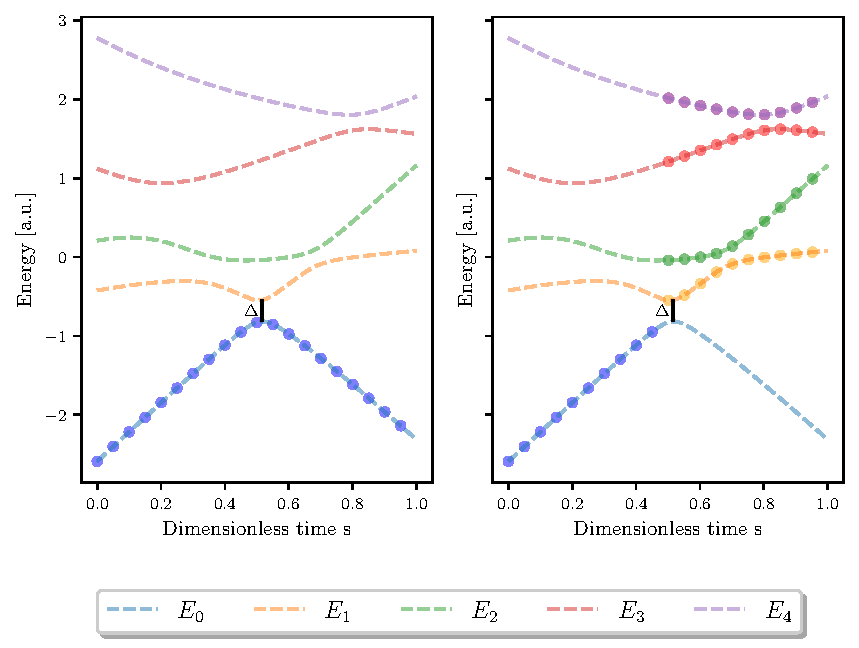
\includegraphics[width=\textwidth]{Figures/Eigenenergies.pdf}
    \caption{Eigenenergies of a random Hamiltonian as function of dimensionless time $s=t/T$ where the problem has been encoded in the ground state. \textbf{Left}: when adiabatic conditions are fulfilled, i.e., if the evolution is carried out sufficiently slowly, then our system evolves continuously in time along the ground state. \textbf{Right}: when the evolution is carried out not fulfilling the adiabatic conditions, it could happen that we end up in a different eigenstate if our system absorbs enough energy to jump to next level over the evolution, something that is more likely to happen close to the minimum gap in the minimum gap $\Delta$. If that happens we would end up in a different eigenstate of the target Hamiltonian which does not encodes the optimal solution.}
    \label{fig:Eigenenergies}
\end{figure}
\newpage
Quoting Goldstone \textit{et al.}\,\cite{Farhi2000QuantumEvolution},
\begin{displayquote}
\textit{...if the gap between the two lowest levels, $E_{1} - E_{0}$, is strictly greater than zero for all $0 \leq t \leq T$, then}
\end{displayquote}
\begin{equation}
    \lim_{T\longrightarrow \infty} | \braket{0(t=T) | \psi(t=T)}| = 1
\end{equation}
Equivalently, the probability of being in the ground state, $\ket{0(t=T)}$, of the target Hamiltonian $\mathcal{H}_{f}$ at the end of evolution is 1 if and only if the total time required for the evolution is infinite. Otherwise, the probability of being in the ground state is
\begin{equation}
    || \braket{0(t=T) | \psi(t=T)}||^{2} = 1 - \epsilon^{2}
\end{equation}
where $|\epsilon| \leq 1$ takes into account the error due to the adiabatic approximation, $\dot{U}(s) \simeq 0$.
%%%%%%%%%%%%%%%%%%%%%%%%%%%%%%%%%%%%%%%%%%%%%%%%%%%%%%%%%%%%%%%%%%%%%%%%%%%%%%%%%%%%%%%%%%%%%%%%%%%%%%%%%%
%     1.2 ADIABATIC THEOREM
%%%%%%%%%%%%%%%%%%%%%%%%%%%%%%%%%%%%%%%%%%%%%%%%%%%%%%%%%%%%%%%%%%%%%%%%%%%%%%%%%%%%%%%%%%%%%%%%%%%%%%%%%%
\subsection{The Adiabatic Theorem: A Formal Derivation}
We start by writing down the Schrödinger equation
\begin{equation}
    i\hbar \frac{\partial \ket{\psi(t)}}{\partial t} = \mathcal{H}(t)\ket{\psi(t)}
\end{equation}
We assume that the instantaneous spectrum of $\mathcal{H}(t)$ is discrete and non-degenerate
\begin{equation}
\label{eq:Hamiltonian}
    \mathcal{H}(t) \ket{n(t)} = E_{n}(t)\ket{n(t)}
\end{equation}
where $\ket{n(t)}$ are the instantaneous eigenstates of the Hamiltonian and $E_{n}(t)$ are the eigenenergies labelled by $n$. Notice that we can label the eigenenergies with a single index because the spectrum is discrete and non-degenerate. For a discrete but degenerate spectrum, we would need an extra index to take into account the degeneracy of each state.\\\\
The eigenstates of the Hamiltonian form an orthonormal basis, so we can expand a given state in that basis
\begin{equation}
\label{eq: EigenvectorExpansion}
    \ket{\psi(t)} = \sum_{n}c_{n}(t)e^{i\theta_{n}(t)} \ket{n(t)}
\end{equation}
where
\begin{equation}
    \theta_{n}(t) = -\frac{1}{\hbar}\int_{0}^{t}E_{n}(t^{\prime})dt^{\prime}
\end{equation}
is the dynamic phase.\\
Substituting Eq.\,\eqref{eq: EigenvectorExpansion} into the Schrödinger equation yields
\begin{equation}
    \sum_{n}\left[\dot{c}_{n}(t)\ket{n(t)} + c_{n}(t)\ket{\dot{n}(t)}\right]e^{i\theta_{n}(t)} = 0
\end{equation}
Multiplying by $\bra{m(t)}$
\begin{equation}
\label{eq:Coefficients}
    \dot{c}_{m}(t) = - \sum_{n}c_{n}\braket{m(t)|\dot{n}(t)}e^{i\left(\theta_{n}(t) - \theta_{m}(t)\right)}
\end{equation}
We need to re-write $\braket{m(t)|\dot{n}(t)}$ in terms of the Hamiltonian's derivative using Eq.\,\eqref{eq:Hamiltonian}. If we derive that expression with respect to time, we find
\begin{equation}
    \frac{\partial \mathcal{H}(t)}{\partial t}\ket{n(t)} + \mathcal{H}(t)\frac{\partial \ket{n(t)}}{\partial t} = \frac{\partial E_{n}(t)}{\partial t} \ket{n(t)} + E_{n}(t)\frac{\partial \ket{n(t)}}{\partial t} 
\end{equation}
Multiplying the last expression by $\bra{m(t)}$, with $m\neq n$,
\begin{equation}
    \braket{m(t)|\frac{\partial\mathcal{H}(t)}{\partial t}|n(t)} + E_{m}(t)\braket{m(t)|\dot{n}(t)} = E_{n}(t)\braket{m(t)|\dot{n}(t)}
\end{equation}
Finally,
\begin{equation}
    \braket{m(t)|\dot{n}(t)} = \frac{1}{E_{n}(t)-E_{m}(t)}\braket{m(t)|\frac{\partial \mathcal{H}(t)}{\partial t}|n(t)}
\end{equation}
Substituting into Eq.\,\eqref{eq:Coefficients} and defining $g_{nm}(t)\equiv E_{n}(t) - E_{m}(t)$ as the energy difference as a function of time $t$ between the eigenstates $\ket{m(t)}$ and $\ket{n(t)}$ leads to
\begin{equation}
\label{eq:GeneralCoefficientsNoadiabaticApprox}
    \dot{c}_{m}(t) = -c_{m}(t) \braket{m(t)|\dot{m}(t)} - \sum_{n\neq m} c_{n}(t)\frac{\braket{m(t)|\dot{\mathcal{H}}(t)|n(t)}}{g_{nm}(t)}e^{i\left(\theta_{n}(t) - \theta_{m}(t)\right)}
\end{equation}
Adiabatic evolution is ensured if the coefficients $c_{n}(t)$ evolve independently from each other, i.e., if their dynamical equations do not couple. Mathematically,
\begin{equation}
    \max_{0 \leq t \leq T} \abs{\frac{\braket{m(t)|\dot{\mathcal{H}}(t)|n(t)}}{g_{nm}(t)}} \ll \min_{0\leq t \leq T} \abs{g_{nm}(t)}
\end{equation}
where $T$ is the total evolution time.\\ 
Under the adiabatic approximation the coupling term tends to zero, that is,
\begin{equation}
    \sum_{n\neq m} c_{n}\frac{\braket{m(t)|\dot{\mathcal{H}(t)}|n(t)}}{g_{nm}(t)}e^{i\left(\theta_{n}(t) - \theta_{m}(t)\right)} \to 0
\end{equation}
Therefore, equation Eq.\,\eqref{eq:GeneralCoefficientsNoadiabaticApprox} turns into
\begin{equation}
    \dot{c}_{m}(t) = -c_{m}(t)\braket{m(t)|\dot{m}(t)}
\end{equation}
whose solution is
\begin{equation}
    c_{m}(t) = c_{m}(0)e^{i\gamma_{m}(t)}
\end{equation}
where
\begin{equation}
    \gamma_{m}(t) = i\int_{0}^{t}\braket{m(t^{\prime})|\dot{m}(t^{\prime})}dt^{\prime} \quad \gamma_{m}\in \mathbb{R}
\end{equation}
is the Berry's phase.
%%%%%%%%%%%%%%%%%%%%%%%%%%%%%%%%%%%%%%%%%%%%%%%%%%%%%%%%%%%%%%%%%%%%%%%%
%       TOTAL EVOLUTION TIME
%%%%%%%%%%%%%%%%%%%%%%%%%%%%%%%%%%%%%%%%%%%%%%%%%%%%%%%%%%%%%%%%%%%%%%%%
\subsection{Total Evolution Time $T$}
In previous sections we stated that under a sufficiently slowly Hamiltonian evolution the adiabatic theorem is satisfied. In this section we define what "slow" means by deriving an expression to estimate the total time $T$ required for the adiabatic evolution. We also demonstrate that the total time not only depends on the energy gap between the ground state and the first excited state but also on the term $\braket{m(s)|d\mathcal{H}(s)/ds|n(s)}$.\\\\
We start by re-writing Eq.\,\eqref{eq:GeneralCoefficientsNoadiabaticApprox} in terms of the normalised time $s = \frac{t}{T}$ and the Berry's phase.
\begin{equation}
    e^{i\gamma_{m}(sT)}\frac{1}{T}\frac{\partial }{\partial s}\left[c_{m}(sT)e^{-i\gamma_{m}(sT)}\right] = -\sum_{n\neq m} c_{n}(sT) \frac{\braket{m(sT)|\dot{\mathcal{H}}(sT)|n(sT)}}{g_{nm}(sT)}e^{-i\left(\theta_{n}(sT) - \theta_{m}(sT)\right)}
\end{equation}
Notice we have added two Berry's phases terms with opposite sign so they cancel out. Integrating the last equation and re-arranging terms leads to
\begin{equation}
\label{eq:Coeff}
    c_{m}(s)e^{-i\gamma_{m}(s)} = c_{m}(0) - \sum_{n\neq m}\int_{0}^{s} ds^{\prime}\frac{F_{nm}(s^{\prime})}{g_{nm}(s^{\prime})}e^{-iT\int_{0}^{s^{\prime}}ds^{\prime\prime}\left(g_{nm}(s^{\prime\prime})\right)}
\end{equation}
This equation expresses the coefficient $c_{n}(s)$ in terms of its initial value $c_{n}(0)$ and a summation term that keep the rest of coefficients $c_{m}(s)$ with $m\neq n$, where
\begin{equation}
\label{eq:Fnm}
    F_{nm}(s) = c_{n}(s)\braket{m(s)|\dot{\mathcal{H}}(s)|n(s)} e^{-i\gamma_{m}(s)}
\end{equation}
We can express the integrand of Eq.\,\eqref{eq:Coeff} as a difference between two terms,
\begin{align}
\frac{F_{nm}(s^{\prime})}{g_{nm}(s^{\prime})} e^{-iT\int_{0}^{s^{\prime}}\left(ds^{\prime \prime}g_{nm}(s^{\prime\prime}) \right)}= \\
\frac{i}{T}\left[\frac{d}{ds^{\prime}}\left(\frac{F_{nm}(s^{\prime})}{g^{2}_{nm}(s^{\prime})}e^{-iT\int_{0}^{s^{\prime}}\left(ds^{\prime \prime}g_{nm}(s^{\prime\prime}) \right)}\right) - e^{-iT\int_{0}^{s^{\prime}}\left(ds^{\prime \prime}g_{nm}(s^{\prime\prime}) \right)} \frac{d}{ds^{\prime}}\left(\frac{F_{nm}(s^{\prime})}{g_{nm}(s^{\prime})}\right)\right] 
 \end{align}
 Substituting the previous result into Eq.\,\eqref{eq:Coeff} leads to
 \begin{equation}
 \begin{split}
      c_{m}(s)e^{-i\gamma_{m}(s)} & = c_{m}(0) + \frac{i}{T}\Biggr[\frac{F_{nm}(0)}{g^{2}_{nm}(0)} - \frac{F_{nm}(s)}{g^{2}_{nm}(s)}e^{-iT\int_{0}^{s}ds^{\prime}g_{nm}(s^{\prime \prime})} \\
      & + \int_{0}^{s}ds^{\prime} e^{-iT\int_{0}^{s^{\prime}}\left(ds^{\prime \prime}g_{nm}(s^{\prime\prime}) \right)} \cdot \frac{d}{ds^{\prime}}\left(\frac{F_{nm}(s^{\prime})}{g_{nm}(s^{\prime})}\right)\Biggr]
\end{split}
\end{equation}
 Assuming the energy gap does not vanish when $T \rightarrow \infty$ and that $d\{F_{nm}(s^{\prime})/g_{nm}^{2}(s^{\prime})\}/ds^{\prime}$ is integrable for all $s \in [0,1]$, the Riemann-Lebesgue lemma [\textbf{REFERENCE Tiene sentido ponerla? es un libro}] guarantees that the last integral vanishes in the limit $T \rightarrow \infty$. So
  \begin{align}
  \label{eq:cm}
     c_{m}(s)e^{-i\gamma_{m}(s)} = c_{m}(0) + \frac{i}{T}\left[\frac{F_{nm}(0)}{g^{2}_{nm}(0)} - \frac{F_{nm}(s)}{g^{2}_{nm}(s)}e^{-iT\int_{0}^{s}ds^{\prime}g_{nm}(s^{\prime \prime})}\right] 
 \end{align}
 Under the adiabatic conditions there are not mixing terms, i.e., the coefficient $c_{n}(s)$ does not depend on the rest of coefficients. Mathematically,
\begin{equation}
    c_{m}(m) = c_{0}(s)e^{i\gamma_{m}(s)}
\end{equation}
Therefore, we can simplify Eq.\,\eqref{eq:Fnm}
\begin{equation}
    F_{nm}(s) = c_{n}(0)\braket{m(s)|\dot{\mathcal{H}}|n(s)} e^{-i\left[\gamma_{m}(s) - \gamma_{n}(s)\right]}
\end{equation}
 With that simplification we can estimate the total time for an adiabatic evolution by imposing a condition that minimises the second term of Eq.\,\eqref{eq:cm}
 \begin{equation}
     T \gg \frac{F}{g^{2}}
 \end{equation}
 where
 \begin{align}
     F = \max_{0 \leq s \leq 1} \left|c_{n}(0)\braket{m(s)|\frac{d\mathcal{H}(s)}{ds}| n(s)}\right| \\
     g = \min_{0 \leq s \leq 1} |g_{nm}(s)|
 \end{align}
%-------------------------------------------------------------------------------------
% QUANTUM ANNEALING
%---------------------------------------------------------------------------------------
\section{Quantum Annealing}
\textit{Quantum annealing} (QA) takes its name from a classical heuristic algorithm named s\textit{imulated annealing} (SA), see Appx.\,\ref{AppendixB}. It is a particularization of AQC where the Hamiltonian is the Ising's Hamiltonian
\begin{equation}
    \mathcal{H}(s) = -\sum_{ij}\mathcal{J}_{ij}\sigma_{i}^{z}\sigma_{j}^{z} - h\sum_{i}\sigma_{i}^{z}
\end{equation}
Spin information is given by the eigenvalues of Pauli Z-operators $\sigma^{z}$, where the possibles outcomes are $\{-1,1\}$ corresponding to the eigenvectors $\{\ket{\uparrow},\ket{\downarrow}\}$, respectively.\\\\
Notice we are mapping our mathematical problem into a physical problem. Solving a problem in a classical computer demands computational resources of it, however if the problem is mapped into a physical problem, then it is the nature evolving in time according to the laws of physics what solves the problem.\\\\
We also need an initial Hamiltonian whose ground state is easy to compute and prepare, e.g.,
\begin{equation}
    \mathcal{H}(s) = -\sum_{i}^{n}\sigma_{i}^{x}
\end{equation}
with ground state $\ket{+}^{n}$. This ground state considers all the possible configurations of our systems with a uniform distribution.\\\\
The annealing schedule between these Hamiltonians is given by
\begin{equation}
    \mathcal{H}(s) = -\sum_{ij}\mathcal{J}_{ij}\sigma_{i}^{z}\sigma_{j}^{z} - h\sum_{i}\sigma_{i}^{z} - \Gamma(s)\sum_{i}\sigma_{i}^{x}
\end{equation}
where $\Gamma(s)\sum_{i}\sigma_{i}^{x}$ represents the quantum fluctuations -- single-spin flip -- and $\Gamma(s)$ plays the same role as temperature in SA. The way of controlling the quantum fluctuations depends on the hardware we are using. The hardware implementation and topology of the quantum computer we have used in the present work is discussed in Appx.\,\ref{AppendixC}.\\\\
Initially, at $s \rightarrow 0$, the dominating term is $\Gamma(s)\sum_{i}\sigma_{i}^{x}$ because $\Gamma(s)$ takes a large value, but at later times $s \rightarrow 1$, $\Gamma(s)$ takes a value close to zero so the dominating Hamiltonian is $\mathcal{H}(s) = -\sum_{ij}\mathcal{J}_{ij}\sigma_{i}^{z} - h\sum_{i}\sigma_{i}^{z}$ which is the Hamiltonian we are interested in, as it contains the solution to our problem encoded in the ground state.
%------------------------------------------------------------------
% Formlation of QUBO problems
%------------------------------------------------------------------
\subsection{Formulation of Quadratic Unscontrained Binary Optimization Problems}
\begin{definition}[\textit{Quadratic Unconstrained Binary Optimization} (QUBO)]
   A Quadratic unconstrained binary optimization problem can be written as
\begin{equation}
    \min_{\vec{x}}\vec{x}^{T}Q\vec{x}
\end{equation}
where $n$ is the total number of binary variables, $\vec{x}\in\{0,1\}^{n}$ are the binary variables of the problem and $Q$ is an $n\times n$ matrix whose entries encodes our problem.
\end{definition}
Notice that the Ising Hamiltonian uses the binary variables $s_{i} = \{-1,1\}$ but QUBO problems are formulated with the binary variables $x_{i} = \{0,1\}$. Both formulations are equivalent if we consider the following mapping between Ising and QUBO variables
\begin{equation}
    s_{i} = 2x_{i} -1
\end{equation}
When writing a given combinational problem into its QUBO formulation the constraints have to be mapped into its binary form. The following table summarises some of the most common binary constraints and how to map them into QUBO formulation.
\begin{table}[H]
\centering
\begin{tabular}{ |c||c| }
 \hline
 \textbf{Constraint} & \textbf{QUBO penalty} \\
 \hline
 $x_{1}=x_{2}$ & $P\left(x_{1} + x_{2} -2x_{1}x_{2}\right)$  \\
 $x_{1}\leq x_{2}$ &  $P\left(x_{1} -x_{1}x_{2}\right)$   \\
 $x_{1} + x_{2} = 1$ & $P\left(1-x_{1}-x_{2}+2x_{1}x_{2}\right)$ \\
 $x_{1} + x_{2} \leq 1$    & $P\left(x_{1}x_{2}\right)$ \\
$x_{1} + x_{2} \geq 1$ &   $P\left(1-x_{1}-x_{2}+x_{1}x_{2}\right)$ \\
 \hline
\end{tabular}
\caption{Mapping of common binary constraints into QUBO formulation.}
\end{table}
There are constraints that require of additional binary variables -- slack variables -- in order to reformulate them into QUBO. These type of constraints can be written as a binary expansion as follows. Suppose we have the following constraint,
\begin{equation}
    \sum_{i}w_{i}x_{i}\leq W
\end{equation}
where the $W$ for simplicity is an integer value. The QUBO penalty of that constraint is
\begin{equation}
    P \left(\sum_{k=0}^{M}c_{k}y_{k} - \sum_{i}w_{i}x_{i} \right)^{2} \\
\end{equation}
where $M = \lfloor\log_{2}{W}\rfloor$ is the floor binary logarithm of $W$, $c_{k} = 2^{k}$ is a binary expansion coefficient and $c_{M} = W + 1 - 2^{M}$ is the last term of that binary expansion. \\\\
Notice that slack variables have to be included in our problem which implies the size of our problem is increased by the number of slack variables. Classically, the increment in the number of variables just affects the complexity of the problem but for a quantum annealer this increment could imply that the problem is not solvable with the current size of annealers. If that is the case, we have to simplify the model until the annealer is able to handle it, or we have to look for other techniques such as hybrid methods, see Ch.\,\ref{Chapter3}, to tackle the problem.

%------------------------------------------------------------------
% Two Heirs Problem
%------------------------------------------------------------------
\subsection{Example: Two Heirs Problem}
 As an example suppose we are given a 3-binary QUBO problem where each variable $x_{i} \in \{0,1\}$ represents an asset with an associated value $v_{i}$.\\
\begin{table}[h]
\label{tab:Assets}
\centering
\begin{tabular}{ |c | c| }
  \hline			
  \textbf{Index} & \textbf{Value}  \\
    \hline		
   0 & 1\\
       \hline		
   1 & 3\\
       \hline		
   2 & 1\\
        \hline	
\end{tabular}
\caption{Two heirs example given three assets.}
\end{table}
\\
We have to assign the assets to two heirs, Alice and Bob -- represented by $\{0,1\}$ in the QUBO formulation and by $\{-1,1\}\equiv \{\uparrow, \downarrow\}$ in the Ising formulation, respectively -- so that the difference between the value each heir receives is minimum, which represents our cost function
\begin{equation}
    f(x_{0}, x_{1}, x_{2}) = \left[\text{Alice}(x_{0}, x_{1}, x_{2}) - \text{Bob}(x_{0}, x_{1}, x_{2})\right]^{2} = \left[\sum_{i}\left((1-x_{i})\cdot v_{i} - x_{i}\cdot v_{i}\right)\right]^{2}
\end{equation}
Notice we are not interested in the sign of our cost function. Therefore, to avoid dealing with signs we take the square of the difference so we know we are minimising a positive quantity.\\\\
Expanding the square we arrive at the QUBO formulation, $\vec{x}^{T}Q\vec{x}$. Notce that for $x_{i} \in \{0,1\}$ the following relation holds $x_{i}=x_{i}^{2}$. 
\begin{align}
    \left[\sum_{i}\left((1-x_{i})\cdot v_{i} - x_{i}\cdot v_{i}\right)\right]^{2} = \sum_{i=0}^{2}\sum_{j\neq i}x_{i}v_{i}v_{j}x_{j} - x_{i}v_{i}v_{j}x_{i} - x_{j}v_{i}v_{j}x_{j}
\end{align}
Therefore, the QUBO matrix of this example is
\begin{equation}
Q= 
    \begin{bmatrix}
           0 & v_{1}v_{2} & v_{1}v_{3}\\
           v_{2}v_{1} & 0 & v_{2}v_{3}\\
           v_{3}v_{1}& v_{3}v_{2} & 0\\
         \end{bmatrix}
\end{equation}
We can add the contribution of mixed indices of the bottom triangular in the upper triangular part of the matrix
\begin{equation}
Q= 
    \begin{bmatrix}
           0 & 2v_{1}v_{2} & 2v_{1}v_{3}\\
           0 & 0 & 2v_{2}v_{3}\\
           0& 0 & 0\\
         \end{bmatrix}
\end{equation}
Notice that we also have dropped the constant terms as they only shift the minimum value but do not affect our solution, i.e., the minimum value of our cost function is going to change but the configuration that leads to that minimum remains the same.\\\\
We now encode our solution into an Ising Hamiltonian $\mathcal{H}_{f}$ by using the mapping between QUBO and Ising variables and we initialise the evolution with the Hamiltonian $\mathcal{H}_{i} = -\sum_{i}^{n}\sigma_{i}^{x}$ whose ground state is $\ket{+}^{n}$. The  Ising formulation of the two heirs example is
\begin{align}
\mathcal{H} = \sum_{i}\sum_{j}x_{i}Q_{ij}x_{j} = \sum_{i}\sum_{j}\left( \frac{s_{i}-1}{2}\right)Q_{ij}\left(\frac{s_{j}-1}{2}\right) = \\
\sum_{i}\sum_{j}\left[\frac{1}{4}\left(s_{i}Q_{ij}s_{j}\right) - \frac{1}{2}\left(s_{i}Q_{ij}\right) + \frac{1}{4}Q_{ij}\right]
\end{align}
If the evolution is carried out under the adiabatic conditions,
\begin{equation}
    \mathcal{H}(s) = -\sum_{ij}\mathcal{J}_{ij}\sigma_{i}^{z}\sigma_{j}^{z} - h\sum_{i}\sigma_{i}^{z} - \Gamma(s)\sum_{i}\sigma_{i}^{x}
\end{equation}
then we end up in $\mathcal{H}_{f}$ with one of the following solutions
\begin{align}
    \mathcal{H}_{f}\ket{g(s=1)} = E_{g}(s=1)\ket{\downarrow\uparrow\downarrow} \\
    \mathcal{H}_{f}\ket{g(s=1)} = E_{g}(s=1)\ket{\uparrow\downarrow\uparrow}
\end{align}
This means that we get a global minimum value $E_{g}(s=1)$ associated with the ground states $\{\ket{\downarrow\uparrow\downarrow},\ket{\uparrow\downarrow\uparrow}\}$. This is because in this case, the problem has a degenerate ground state and the eigenvectors correspond to different configurations of our binary variables that lead to the same absolute minimum value $E_{g}(s=1)$. Intuitively, if a solution $\ket{\uparrow\downarrow\uparrow}$ indicates that Alice receives assets with indices $[0,2]$ and Bob receive the asset with index $[1]$, the opposite is a solution $\ket{\downarrow\uparrow\downarrow}$ with the same cost, i.e., Bob receives assets with indices $[0,2]$ and Alice receives the asset with index $[1]$.
%%%%%%%%%%%%%%%%%%%%%%%%%%%%%%%%%%%%%%%%%%%%%%%%%%%%%%%
\section{Circuit Based AQC: A First Approach}
In this section we sketch the idea of how to reproduce AQC in the gate model of computation with arbitrary precision. For a deeper understanding see Ref.\,\cite{Farhi2014AAlgorithm}.\\\\
From the definition of the exponential of an operator $\hat{A}$
\begin{equation}
    e^{\hat{A}}=\lim_{n\rightarrow \infty}\left( 1 + \frac{\hat{A}}{n}\right)^{n}
\end{equation}
we can compute the exponential of a sum of operators as
\begin{equation}
    e^{\hat{A}+\hat{B}}=\lim_{n\rightarrow \infty}\left( 1 + \frac{\hat{A} + \hat{B}}{n}\right)^{n} = \lim_{n\rightarrow \infty}\left(e^{\hat{A}/n}e^{\hat{B}/n}\right)^{n}
\end{equation}
Equivalently, by the Suzuki-Trotter expansion of first order 
\begin{equation}
        e^{\left(\hat{A}+\hat{B}\right)\Delta t} = e^{\hat{A}\Delta t}e^{\hat{B}\Delta t} + \mathcal{O}(\Delta t^{2})
\end{equation}
In order to reproduce AQC with gates, we must discretize the time evolution in a set of time steps, $N$, of step size $\Delta t = T/N$,
\begin{align}
    e^{-i\hat{\mathcal{H}}\Delta t} = e^{-i\hat{\mathcal{H}}_{i}\Delta t}e^{-i\hat{\mathcal{H}}_{f}\Delta t} + \mathcal{O}(\Delta t^{2})
\end{align}
where
\begin{equation}
    e^{-i\hat{\mathcal{H}}_{i}\Delta t} = \prod_{k=1}^{N}e^{-i\left(1-\Delta t/k\right)\hat{\mathcal{H}}_{i}}, \quad e^{-i\hat{\mathcal{H}}_{f}\Delta t} = \prod_{k=1}^{N}e^{-i\left(1-\Delta t/k\right)\hat{\mathcal{H}}_{i}}
\end{equation}
represent the time discretization of the initial and target Hamiltonians respectively. \\\\
Hence we can decompose the adiabatic evolution operator $\hat{U}(T,0) = e^{-i\mathcal{H}(t)}$ in a product of exponential
\begin{equation}
    \ket{\psi(t = T)} = \hat{U}(T,0)\ket{\psi(t = 0)} \simeq \prod_{k=1}^{N}e^{-i\left(1-\Delta t/k\right)\hat{\mathcal{H}}_{i}}e^{-i\left(1-\Delta t/k\right)\hat{\mathcal{H}}_{i}}\ket{\psi(t = 0)} 
\end{equation}
In the limit $N \rightarrow \infty$ the gate model reproduces exactly the adiabatic evolution.
%%%%%%%%%%%%%%%%%%%%%%%%%%%%%%%%%%%%%%%%%%%%%%%%%%%%%%%